\documentclass{article}
\usepackage{graphicx}

% Title
\title{CamelidCoin: A Model Network For Distributed LLM Computation and Training}

% Author
\author{Dylan Dunn}
\date{May 5, 2023}

\begin{document}

\begin{titlepage}
    \centering
    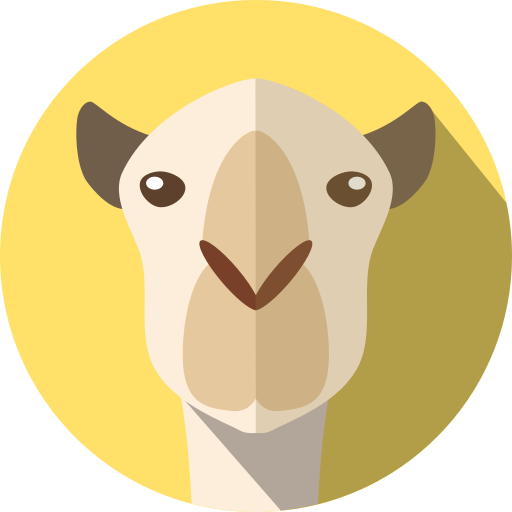
\includegraphics[width=0.5\textwidth]{logoLarge.png}\par\vspace{1cm}
    {\fontsize{40}{48}\selectfont\scshape CamelidCoin\par}
    \vspace{1cm}
    {\scshape\Large A Blockchain-based Model for Trustless Distributed LLM Computation and Training. \par}
    \vspace{2cm}
    {\Large\itshape Dylan Dunn\par}
    \vfill
    {\large May 5, 2023\par}
  \end{titlepage}
  

\section{Abstract}
CamelidCoin is a trustless, incentive-based blockchain protocol designed for distributed auto-regressive large language model (LLM) computation and training. 
The system is built on a peer-to-peer network where lightweight clients can submit input for completion by a large pool of compute nodes. 
In exchange for their work, the compute nodes are compensated by the client. 
To ensure the validity of the output from these compute nodes, we propose a new algorithm called RASTiC, which can be completed either by the client or other compute nodes. 
This algorithm quickly verifies the output's authenticity with near certainty. 
Additionally, throughout the paper, we will detail the protocol's structure and specifics
Our protocol works off of the original peer-to-peer electronic cash system proposed by Satoshi Nakamoto's Bitcoin and modifies it to fit our use case. 
We will also discuss current challenges and limitations with our current protocol.

\section{Introduction}
\subsection{Related Work}

\section{Technical Overview}
\subsection{Network}
\subsubsection{Peer Discovery}
\subsubsection{Messaging Protocol}

\subsection{Wallet}
\subsubsection{Keypair Creation}
\subsubsection{Public Address}

\subsection{Transaction}
\subsubsection{Structure}
\subsubsection{Verification}

\subsection{Block}
\subsubsection{Structure}

\subsection{Chain}

\subsection{Job}
\subsection{Job Pool}
\subsection{Dispute Resolution}

\subsection{RASTiC Verification Algorithm}
\subsubsection{Problem Statement and Motivation}
\subsubsection{Implementation and Methodology}
\subsubsection{Performance Evaluation}
\subsubsection{Potential Attacks and Exploits}

\section{Challenges and Limitations}
\subsection{Privacy}

\section {Future Aspirations}
\subsection{Distributed Training}
\subsection{Proof of Stake}
\subsection{Improved Privacy}    

\section {Conclusion}

\end{document}                                                          